\subsection{One Illustrative Operating Point: a 30\% Granule Overhead}
\label{sec:rd_illustrative}

The tables that follow evaluate the comparison at
$\gamma_{\mathrm{tile}}=1.30$, the illustrative overhead scenario of
Section~\ref{sec:overhead}. Every verdict in them is the curve of
Table~\ref{tab:gamma_continuous} read at one abscissa: HEALPix is the
smaller representation exactly where $1.30$ exceeds that target's
$\gamma_\star$, which is why the sign changes between $10^{-3}$ and
$3\times10^{-3}$ and nowhere else. In sizes: if the native product is
stored with $30\%$ of padding and metadata, the Clough--Tocher carrier is
$1.59$ times its size at the tightest tolerance and $0.72$ times at the
loosest. Each entry of Tables~\ref{tab:storage_at_rmse}
and~\ref{tab:error_at_size} is a per-region HPX/UTM ratio with the
oracle-best codec chosen per region and per grid, the UTM side carrying
$\gamma_{\mathrm{tile}}=1.3$, so a value below one favours HEALPix; the
median is over the $n$ evaluable regions of 40, with the range in
brackets; $p$ is a two-sided Wilcoxon test on the log ratio, and
$p^{\mathrm{Holm}}$ corrects over the family of eight targets the two
tables report together. The last column follows the corrected test: a
target it does not separate at the $5\%$ level is marked inconclusive
whatever the side of its median.

\begin{table}[t]
\centering
\caption{Per-scene HPX/UTM compressed-size ratio at constant reconstruction RMSE (oracle-best codec chosen independently per scene per side; UTM already includes the assumed $\gamma_{\mathrm{tile}}=1.30$ Sentinel-2/MGRS granule-overhead scenario). Ratio $<1$ favors HEALPix. Median and [min, max] across the $n$ evaluable scenes (of 7). $p_{\mathrm{raw}}$: exact two-sided Wilcoxon signed-rank test on this target alone. $p_{\mathrm{Holm}}$: Holm-adjusted across the full family of 9 targets tested in Tables~\ref{tab:storage_at_rmse}--\ref{tab:error_at_size}; treat all targets here as exploratory, not confirmatory.}
\label{tab:storage_at_rmse}
\begin{tabular}{lrrlrr}
\toprule
Target RMSE & $n$ & Median ratio & Range & $p_{\mathrm{raw}}$ & $p_{\mathrm{Holm}}$ \\
\midrule
$10^{-4}$ & 7 & 1.59 & [1.26, 1.71] & 0.016 & 0.141 \\
$3\times10^{-4}$ & 7 & 1.47 & [0.61, 1.68] & 0.078 & 0.234 \\
$10^{-3}$ & 7 & 1.24 & [0.94, 1.89] & 0.047 & 0.188 \\
$3\times10^{-3}$ & 5 & 0.80 & [0.54, 1.24] & 0.625 & 1.000 \\
$10^{-2}$ & 5 & 0.91 & [0.68, 2.02] & 0.625 & 1.000 \\
\bottomrule
\end{tabular}
\end{table}


At matched RMSE (Table~\ref{tab:storage_at_rmse}), native UTM is ahead at
the three tightest targets: HEALPix needs $1.23$--$1.59\times$ the size of
the native product under the illustrative overhead from $10^{-3}$ to
$10^{-4}$, with Holm-adjusted $p\le0.016$. The order reverses at
$10^{-2}$, where HEALPix needs $0.72\times$ that size over the 32 regions
whose contrast admits the target (Holm-adjusted $p<10^{-4}$). Between
them, $3\times10^{-3}$ lies near parity (median $0.92$, $n=37$) and is the
only reported target that fails correction ($p^{\mathrm{Holm}}=0.14$); it
is reported as inconclusive, since no equivalence margin has been
defined. Appendix~\ref{app:censoring} shows that keeping the excluded
regions as bounds would change no verdict. In
Table~\ref{tab:error_at_size} the budget is a fraction of the shared raw
HEALPix tile size, \SI{4194304}{\byte}, the UTM side receives that budget
divided by $\gamma_{\mathrm{tile}}$, and the ratio compared is of
reconstruction errors.

\begin{table}[t]
\centering
\caption{Per-region HPX/UTM reconstruction-RMSE ratio at a constant shared storage budget, expressed as a fraction of the shared raw HEALPix tile size (4194304 B); the UTM side receives that budget divided by $\gamma_{\mathrm{tile}}=1.3$. Ratio $<1$ favors HEALPix.}
\label{tab:error_at_size}
\begin{tabular}{lrrrrrl}
\toprule
Target & $n$ & Median ratio & Range & $p$ & $p_{\mathrm{Holm}}$ & Favors \\
\midrule
\bottomrule
\end{tabular}
\\[2pt]\footnotesize Exact/asymptotic two-sided Wilcoxon on $\log$(ratio); $p_{\mathrm{Holm}}$ corrects across the whole family of 0 targets reported in Tables~\ref{tab:storage_at_rmse} and~\ref{tab:error_at_size}.
\end{table}


At matched budget the same regime-dependent pattern holds and every
target survives correction: at the $10\%$ and $5\%$ budgets the
reconstruction RMSE of HEALPix is $4.01\times$ and $1.33\times$ that of
the native product under the illustrative overhead, and at the tightest
budget ($2\%$) the order reverses and HEALPix reaches $0.83\times$ the UTM
RMSE over all 40 regions (Holm-adjusted $p<10^{-4}$).

\begin{figure}[t]
\centering
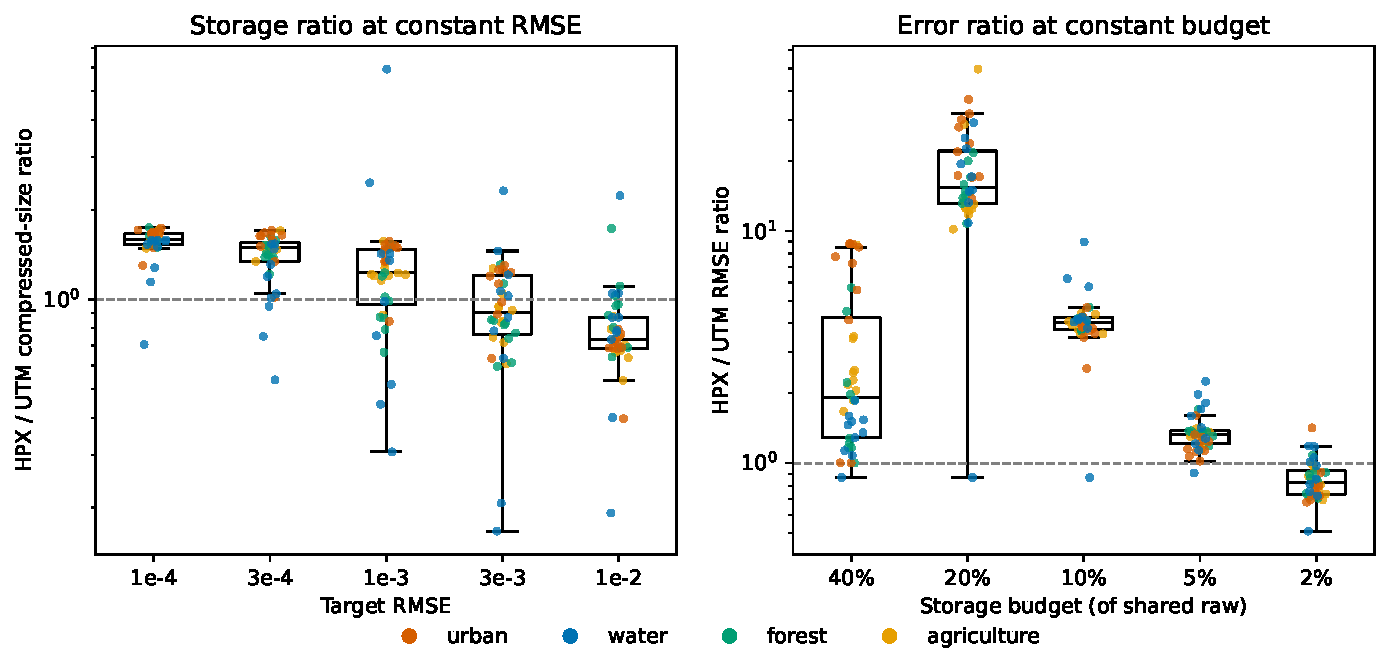
\includegraphics[width=\columnwidth]{figures/fig_ratio_boxplots}
\caption{Per-scene HPX/UTM ratio distributions underlying Tables~\ref{tab:storage_at_rmse}--\ref{tab:error_at_size}, at the illustrative $\gamma_{\mathrm{tile}}=1.30$ of this subsection (oracle-best codec chosen independently per scene, per grid). Left: compressed-size ratio at each target RMSE. Right: RMSE ratio at each target storage budget (log scale). The dashed line at $1.0$ marks parity; values below it favour HEALPix.}
\label{fig:ratio_boxplots}
\end{figure}

Figure~\ref{fig:ratio_boxplots} shows the region-to-region spread behind
each median. Urban regions are the most favourable to UTM at tight
targets (median $1.67$ at $10^{-4}$) and, with agriculture, the most
favourable to HEALPix at the loosest one ($0.70$ and $0.69$ at
$10^{-2}$); water regions produce nearly all the extreme ratios in either
direction, because over near-constant water the compressed files fall
below \SI{10}{kB}, where container overhead is a large share of the total
and any resampling artefact is most of the remaining signal. Medians are
reported for this reason, and individual water-region ratios are treated
as uninformative at the loosest targets. Figure~\ref{fig:rd_comparison}
shows the absolute-value curves, aggregated by median over scenes at each
target; aggregation in absolute bytes mixes scenes of different
difficulty, which the per-scene-ratio protocol was designed to avoid.

\begin{figure}[t]
\centering
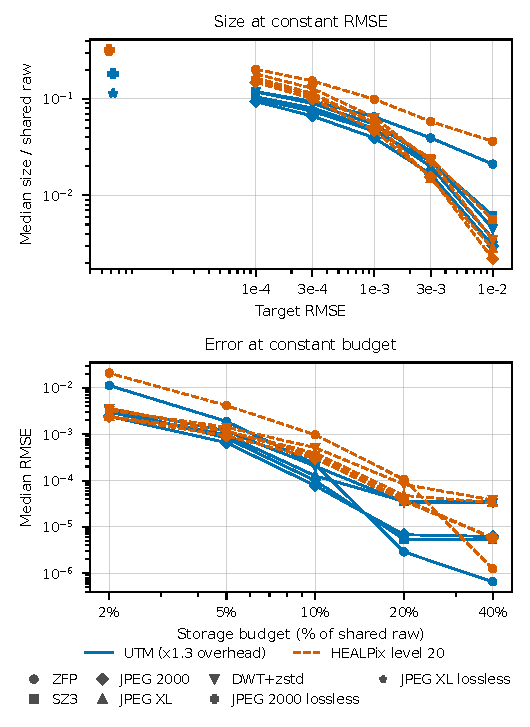
\includegraphics[width=\columnwidth]{figures/fig_storage_at_constant_rmse}
\caption{Rate--distortion curves per codec, native UTM (solid, with the illustrative overhead) and HEALPix level 20 (dashed), one marker per codec: median absolute compressed size at each target RMSE (top, as a fraction of the shared raw tile size) and median RMSE at each storage budget (bottom), over the 40 regions. The lossless codecs are the isolated hollow points.}
\label{fig:rd_comparison}
\end{figure}
